\documentclass[]{article}
\usepackage{lmodern}
\usepackage{amssymb,amsmath}
\usepackage{ifxetex,ifluatex}
\usepackage{fixltx2e} % provides \textsubscript
\ifnum 0\ifxetex 1\fi\ifluatex 1\fi=0 % if pdftex
  \usepackage[T1]{fontenc}
  \usepackage[utf8]{inputenc}
\else % if luatex or xelatex
  \ifxetex
    \usepackage{mathspec}
  \else
    \usepackage{fontspec}
  \fi
  \defaultfontfeatures{Ligatures=TeX,Scale=MatchLowercase}
\fi
% use upquote if available, for straight quotes in verbatim environments
\IfFileExists{upquote.sty}{\usepackage{upquote}}{}
% use microtype if available
\IfFileExists{microtype.sty}{%
\usepackage{microtype}
\UseMicrotypeSet[protrusion]{basicmath} % disable protrusion for tt fonts
}{}
\usepackage[top=3cm,left=3cm,right=3cm]{geometry}
\usepackage{hyperref}
\hypersetup{unicode=true,
            pdftitle={Disease Modeling},
            pdfborder={0 0 0},
            breaklinks=true}
\urlstyle{same}  % don't use monospace font for urls
\usepackage{graphicx,grffile}
\makeatletter
\def\maxwidth{\ifdim\Gin@nat@width>\linewidth\linewidth\else\Gin@nat@width\fi}
\def\maxheight{\ifdim\Gin@nat@height>\textheight\textheight\else\Gin@nat@height\fi}
\makeatother
% Scale images if necessary, so that they will not overflow the page
% margins by default, and it is still possible to overwrite the defaults
% using explicit options in \includegraphics[width, height, ...]{}
\setkeys{Gin}{width=\maxwidth,height=\maxheight,keepaspectratio}
\IfFileExists{parskip.sty}{%
\usepackage{parskip}
}{% else
\setlength{\parindent}{0pt}
\setlength{\parskip}{6pt plus 2pt minus 1pt}
}
\setlength{\emergencystretch}{3em}  % prevent overfull lines
\providecommand{\tightlist}{%
  \setlength{\itemsep}{0pt}\setlength{\parskip}{0pt}}
\setcounter{secnumdepth}{5}
% Redefines (sub)paragraphs to behave more like sections
\ifx\paragraph\undefined\else
\let\oldparagraph\paragraph
\renewcommand{\paragraph}[1]{\oldparagraph{#1}\mbox{}}
\fi
\ifx\subparagraph\undefined\else
\let\oldsubparagraph\subparagraph
\renewcommand{\subparagraph}[1]{\oldsubparagraph{#1}\mbox{}}
\fi

%%% Use protect on footnotes to avoid problems with footnotes in titles
\let\rmarkdownfootnote\footnote%
\def\footnote{\protect\rmarkdownfootnote}

%%% Change title format to be more compact
\usepackage{titling}

% Create subtitle command for use in maketitle
\providecommand{\subtitle}[1]{
  \posttitle{
    \begin{center}\large#1\end{center}
    }
}

\setlength{\droptitle}{-2em}

  \title{Disease Modeling}
    \pretitle{\vspace{\droptitle}\centering\huge}
  \posttitle{\par}
    \author{}
    \preauthor{}\postauthor{}
    \date{}
    \predate{}\postdate{}
  
\usepackage{multirow}
\usepackage{multicol}
\usepackage{booktabs}
\usepackage{xcolor}
\numberwithin{equation}{section}
\counterwithin{figure}{section}
\counterwithin{table}{section}
\usepackage{dcolumn}
\usepackage{rotating}
\usepackage{caption}
\usepackage{amsfonts}
\captionsetup{width=4.5in}
\usepackage{algorithm}

\begin{document}
\maketitle

{
\setcounter{tocdepth}{2}
\tableofcontents
}
\hypertarget{intro}{%
\section{Intro}\label{intro}}

Over May 2011, a strain \emph{Escherichia coli} (\emph{E. coli}) caused
an outbreak of severe illness in Germany, with \textasciitilde{}3,950
affected compared with \textasciitilde{}200 cases a year typically seen.
Of those infected 53 died.

In this - we extend a method presented by Held et al.
(\protect\hyperlink{ref-held_two-component_2006}{2006}) for modeling
parameters of infectious disease counts in a Bayesian framework. Their
method models the count data as a branching Poisson process with a
cyclical endemic parameter.

We then extend their model to incorporate a graph.

\hypertarget{comments}{%
\subsection{Comments}\label{comments}}

Expand and metion general ideas of epidemics spreading \& how we model
them (\textasciitilde{}1 page)

\hypertarget{intro-to-two-component-model}{%
\section{Intro to Two-Component
Model}\label{intro-to-two-component-model}}

Held et al. (\protect\hyperlink{ref-held_two-component_2006}{2006})
presents a stochastic model for the statistical analysis of infectious
disease counts that serves as the basis of the theextended graph model.

The two components of the model are a simple Poisson branching process
with autoregressive parameter \(\lambda\) and a seasonal component fit
with a Fourier series. These components are described as the
``epidemic'' and ``endemic'' components respectively. Additionally, the
two-component model allows for the \(\lambda\) to change over time
allowing for the disease to change infectivity over time.

\hypertarget{two-component-model-notation}{%
\subsection{Two-Component Model
Notation}\label{two-component-model-notation}}

Let \(Z = (Z_0, Z_1, ..., Z_n)\) be the infectious disease counts at
each time step \(t\). The model is then specified through
\(Z_t | Z_{t-1}\).

Each \(Z_t\) is determined as \(Z_t = Y_t + X_t,\ t \in \{1,\dots, N\}\)

Where \(Y_t\) is the epidemic component and \(X_t\) is the endemic
component. The epidemic component is modeled as Poisson distribution as
\[Y_t|Z_{t-1} \sim Pois(\lambda_tZ_{t-1})\]

\[ \lambda_t =  \begin{cases} \lambda^{(1)} & t < \theta_0 \\
\lambda^{(k)}, & \theta_{k} \leq t < \theta_{(k-1)} \\
\lambda^{(K+1)}, & t \geq \theta_K \end{cases}\]

Where \(\lambda_t\) is piecewise constant depending on an unknown number
of changepoints \(K\) and unknown locations
\(\theta_1 < \cdots < \theta_K\).

The endemic component is also Poisson distributed with

\[ X_t \sim Pois(\nu_t)\]

Where \(\log{\nu_t}\) is modeled as a Fourier series:

\[ \log{\nu_t} = \gamma_0 + \sum_{l = 1}^L \big(\gamma_{2l-1}\sin(\rho l t)+\gamma_{2l}cos(\rho l t)\big) \]

\hypertarget{epidemic-component}{%
\subsection{Epidemic Component}\label{epidemic-component}}

The epidemic component is given by:

\[Y_t|Z_{t-1} \sim Pois(\lambda_tZ_{t-1})\]

Where \(\lambda_t\) is the time varing infectivity parameter and
\(Z_{t-1}\) is the the infected count in the previous time step.

We can think of \(\lambda_t\) as the infectivity of the disease at time
\(t\) with an infected person causing new infections as
\(Pois(\lambda_t)\). Since each infected at time \(Z_{t-1}\) generates
new infected i.i.d \(Pois(\lambda_t)\), then \(Z_t\) is the sum of those
random variables which itself is Poisson;
\(\sum_1^{Z_{n-1}}Pois(\lambda_t) = Pois(\lambda_tZ_{n-1})\).

In this model, the \(\lambda_t\) is allowed to vary over time. The
parameter \(\lambda = (\lambda_1,\cdots,\lambda_n)\) is a piecewise
constant function with unknown number of changepoints \(K\) and unknown
location of changepoints \(\theta_1 < \cdots < \theta_K\) with
\(\theta \in \{1,...,n-1\}\). If \(K = 0\) there is no changepoint and
the \(\lambda\) parameter is constant throughout.

\hypertarget{tk-add-references-below}{%
\subsection{TK add references below}\label{tk-add-references-below}}

For constant \(\lambda\), this is known as a Poisson branching process.
For such a process, when \(\lambda > 1\) the process explodes and the
number of infected goes to infinity with probability 1. When
\(\lambda < 1\) then the process ``goes extinct'' or reaches and remains
at 0 with probability 1. Once the process reaches a point where
\(Z_t = 0\), it remains there as there are no more infected to create
new infected at the next time step. When \(\lambda_t > 1\) an
``outbreak'' occurs shown as the spike in the graph between. When
\(\lambda_t < 1\) the outbreak ends.

Allowing \(\lambda_t\) to vary captures many scenarios, for example a
particulary infectious strain of the flu could cause \(\lambda_t\) to
increase above 1 and cause an outbreak. Later, better or new vaccines
and quarentine procedures can cause the overall infectivity to decrease
below 1.

\hypertarget{endemic-component}{%
\subsection{Endemic Component}\label{endemic-component}}

The endemic component in the model plays two roles. It allows capture of
cyclical behaviors in disease counts (e.g.~seasonal flu) and it also
prevents the branching process from going extinct. The endemic count is
modeled as

\[X_t \sim Pois(\nu_t)\]
\[\log{\nu_t} = \gamma_0 + \sum_{l = 1}^L (\gamma_{2l-1}\sin(\rho l t)+\gamma_{2l}cos(\rho l t))\]

That is, \(\log{\nu_t}\) is fit with a Fourier series which can
approximate any function arbitrarily closely. Following, Held et al.
(\protect\hyperlink{ref-held_two-component_2006}{2006}) the series is
computed with \(L = 1\) since it was determined higher order frequencies
were insignificant. That is the truncated series is still flexible
enough to model cylical patterns seen in disease counts.

The parameter can then be fit with a linear regression
\(\log{\nu_t} = s_t\gamma^T\)

where
\(s_t = \langle 1, sin(\rho l t), \gamma_{2l}cos(\rho l t) \rangle\)

\begin{figure}
\centering
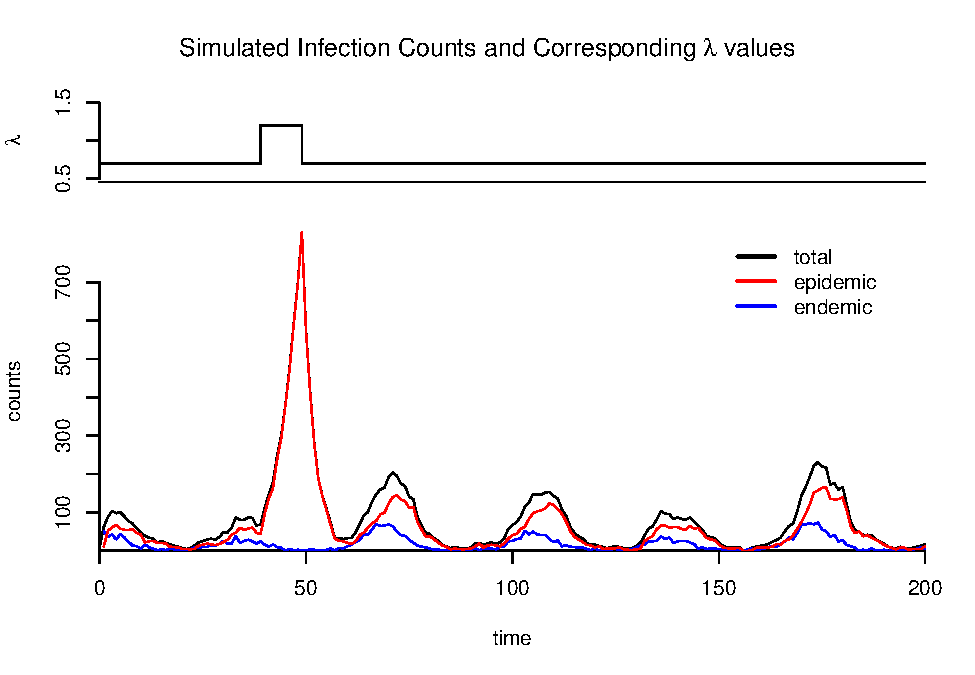
\includegraphics{thesis_draft_files/figure-latex/simulation figure-1.pdf}
\caption{\label{fig:figs}plotting example}
\end{figure}

\hypertarget{likelihood}{%
\subsection{Likelihood}\label{likelihood}}

Then the probability of the full time series \(Z\) given the initial
starting count \(Z_0\) can be factored as a product of the probabilities
of each \(Z_t\) given the previous count \(Z_{t-1}\)

\[P(Z|Z_0,\theta, K, \lambda^{(1)}, \dots, \lambda^{(K+1)}, \gamma_0, \gamma_1, \gamma_2 ) = \prod_{t=1}^b P(Z_t|Z_t{-1}, \theta, K, \lambda^{(1)}, \dots, \lambda^{(K+1)}, \gamma_0, \gamma_1, \gamma_2)\]
Where \(Z_t\) is distributed as sum of the Poisson endemic and epidemic
components
\[Z_t|Z_{t-1}, \theta, K, \lambda^{(1)}, \dots, \lambda^{(K+1)}, \gamma_0, \gamma_1, \gamma_2 \sim Pois(\nu_t + \lambda_tZ_{t-1})\]
where the endemic component \(\nu_t\) is described as
\[\log{\nu_t} = \gamma_0 +  \gamma_{1}\sin(\rho l t)+\gamma_{2}\cos(\rho l t)\]
and \(\lambda_t\) piecewise function is described by
\[ \lambda_t =  \begin{cases} \lambda^{(1)} & t < \theta_0 \\
\lambda^{(k)}, & \theta_{k} \leq t < \theta_{(k-1)} \\
\lambda^{(K+1)}, & t \geq \theta_K \end{cases}\]

\hypertarget{priors}{%
\subsection{Priors}\label{priors}}

The prior values for the \(\gamma\) parameters are Multivariate-Normal
distributed with variance \(3I_3\) to describe the uncertainty.

\[\gamma_i \sim N(0, 3I_3), i \in \{0,1,2\}\]

Since the \(\lambda\) values parameterize a Poisson distribution we set
the prior to be Gamma(1, 1), it's conjugate distribution. If Gamma is
interpreted as the sum of exponentials, then the shape = 1, rate = 1
parameterization represents seeing a single occurence in 1 unit of time
and represents a vague prior.

\[ \lambda^{(k)} \sim Gamma(1, 1),\ k \in \{1, \dots, K + 1\} \]

The number of changepoints \(K\) takes values in \(\{1,\dots,N\}\) where
\(N\) is the total number of time points of counts collected. In the
({\textbf{???}}) paper the number of changepoint is uniformly
distributed \(P(K = k) = 1/N\) representing uncertainty in the number of
changepoints. This is changed to \[K \sim Pois(2)\] representing that
idea that the disease count data is already of interest due to a
potential change in the infectivity of the disease. \(K \sim Pois(2)\)
places the highest mass on \(K = 2\) changepoints which can capture a
spike in disease counts (as seen in the simulated data) before returning
to a baseline endemic rate. It also places mass on \(K = 1\)
(e.g.~capturing a long term decrease in infectivity due to intervention)
and \(K = 3\) changepoints. It also acts as a regularizer to help reduce
overfitting the count time series where each time point is given a
unique \(\lambda_t\) value.

The probability of a specfic location for a change point given the
number of changepoints is uniformly distributed among all the possible
changepoints \[P(\theta|K=k) = \binom{N}{k}^{-1}\] Then the
unnormallized posterior is then the product of the likelihood and the
priors
\[ P(\theta, K, \lambda^{(1)}, \dots, \lambda^{(K+1)}, \gamma_0, \gamma_1, \gamma_2|Z)  \propto \]
\[\prod_{t=1}^N P(Z_t|Z_{t-1},\theta, K, \lambda^{(1)}, \dots, \lambda^{(K+1)}, \gamma_0, \gamma_1, \gamma_2)*P(\theta|K)*P(K)*P(\prod_{k=1}^{K+1}\lambda^{(k)} )*P(\prod_{i=0}^2 \gamma_i)  \]

\hypertarget{graph-data-introduction}{%
\section{Graph Data Introduction}\label{graph-data-introduction}}

We would like to extend our data from a univariate time series of counts
\(Z_t\) to a multiple time series of counts \(Z_{i,t}\) where \(i\) now
indexes separate time series. In this case, \(i\) indexes individual
cities where \(Z_i\) represents the infectious disease counts in city
\(i\). Now, a city \(i\)'s epidemic disease count at time \(t\) is
modelled as a function of both it's counts \(Z_{i,t-1}\) and possibly
other cities counts as well.

This dependency between cities is represented with a fixed graph
\(G_{N_v, E}\) where \(N_v\), the number of vertices in graph is fixed
and equal to the number of cities and \(N_e\) is the number of edges in
the graph, representing dependencies between cities' disease counts. We
call \(V = \{1,\dots,N_v \}\) the vertex set of the graph where \(N_v\)
is the number of cities/individual time series of disease counts, and
\(E(G)\) is a set of unordered pairs of vertices \(\{i,j\}\) where
\(i,j \in V\) and \(i \neq j\) that describes the edges present in graph
\(G\). We represent the edge \(\{i,j\}\) as \(e_{ij}\) and the indicator
\(1[e_{ij}=1]\) if \(\{i,j\} \in E(G)\) and 0 otherwise. For clarity,
the subscripts \(N_v, E\) will be dropped and it's assumed that the true
graph has fixed number of vertices and fixed edges.

\begin{figure}
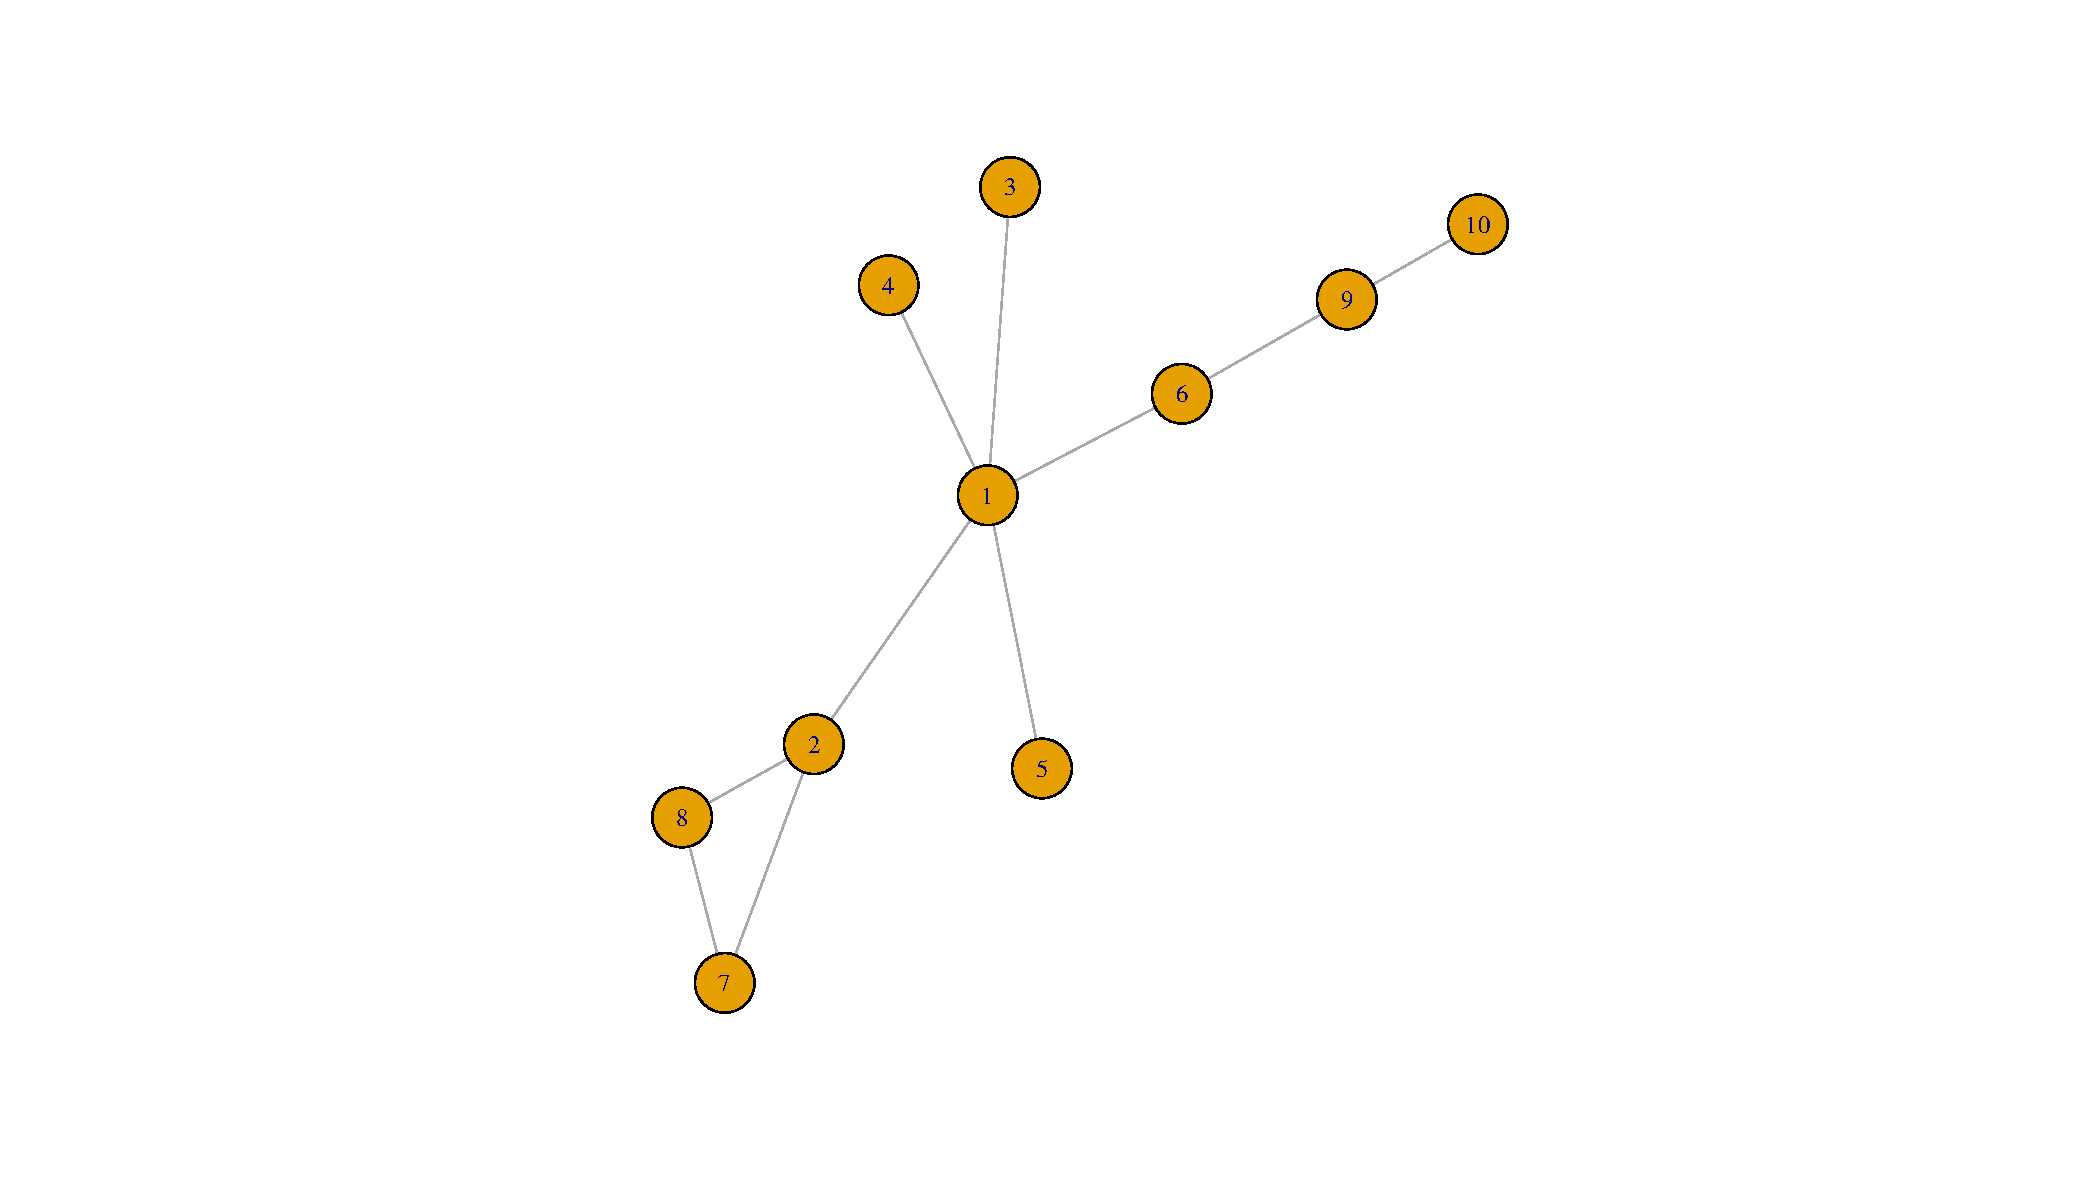
\includegraphics[trim={1 2cm 0 2cm},clip]{thesis_draft_files/figure-latex/unnamed-chunk-1-1} \caption{\label{fig:graph example} A graph configuration. The vertices $i \in \{1,\dots, 10\}$ represent cities each with their own disease counts          $Z_{i,t}$. The edges between the graph represent whether the counts between the cities can affect each other. In this example city 1's disease counts at time $t$ are influenced by both it's own counts and cities 2, 4, 5 and 6's (i.e. every city connected to it) disease counts. City 10's disease counts are only it's own and city 9's.}\label{fig:unnamed-chunk-1}
\end{figure}

We then model the disease count of city \(i\) at time \(t\) as a
function of \(Z_{i,t-1}\) (as before, it's own counts at time \(t-1\))
as well all the counts of the cities \(j\) it is connected to,
\(Z_{j,t-1}\). Then the counts at city \(i\) at time \(t\) are modeled
as \(Z_t|Z_{t-1}, G = X_{i, t} + Y_{i,t}|G\) where
\[X_{i,t}: \text{infected count in city } i \text{ at time step } t \text{, due to endemic factors}   \]
\[Y_{i,t}|G : \text{infected count in city } i \text{ at time step } t \text{, due to epidemic factors}\]
\[Z_{i,t}|G = X_{i,t} + Y_{i,t}|G: \text{infected count in city } i \text{ at time step } t \]
As before we have the epidemic component as
\(X_{i,t} \sim Pois(\nu_t)\). For the epidemic component we now include
the additional counts from connected cities as

\[Y_{i,t}|G \sim ~ Pois\big(\lambda_t*\sum_{j\neq i}^{N_v}Z_{j,t-1}*1[e_{ij}=1]+ \lambda_tZ_{i,t-1}\big)|G \]
Where \(\lambda_t*\sum_{j\neq i}^{N_v}Z_{j,t}*1[e_{ij}=1]\) are the
counts from cities connected to city \(i\).

That is the epidemic component for city \(i\) is the sum of all counts
in every city \(j\) connected to \(i\) in addition to the counts in city
\(i\).

\hypertarget{migration}{%
\subsection{Migration}\label{migration}}

One issue with this model is that connecting two isolated cities
essentially doubles the infectivity parameter, since we include the
counts from both cities. In this formulation a connection between two
cities is equivalent to treating them a single city. To make the model
more realistic, a migration parameter \(m \in (0,1)\) is introduced.

The migration parameter enters into the likelihood as
\[Y_{i,t}|G \sim ~ Pois\big(m*\lambda_t*\sum_{j\neq i}^{N_v}Z_{j,t-1}*1[e_{ij}=1]+ \lambda_tZ_{i,t-1}\big)|G \]
The migration parameter \(m\) is then the fraction of infected in city
\(j\) that can cause infections in city \(i\), where \(m = 1\) is
equivalent to the previous model and all infected in city \(j\) are
counted and \(m = 0\) is no infected are counted and is equivalent to
the cities \(i,j\) not being connected in graph \(G\) (i.e,
\(e_{ij} \notin G\))

\hypertarget{full-likelihood}{%
\subsection{Full Likelihood}\label{full-likelihood}}

\[\prod_{i=1}^{N_v}\prod_{t=1}^N P(Z_{i,t}|Z_{t-1},\theta, K, \lambda^{(1)}, \dots, \lambda^{(K+1)}, \gamma_0, \gamma_1, \gamma_2,G,p)P(\theta|K)P(K)P(\prod_{k=1}^{K+1}\lambda^{(k)} )P(\prod_{i=0}^2 \gamma_i)P(G|p)P(p)\]

\hypertarget{future-extensions}{%
\subsubsection{Future Extensions}\label{future-extensions}}

While this thesis only covers a fixed migration rate, the end goal would
be to model the migration rate as a function of city specific
attributes, e.g.~size of the cities, distance between the cities, if the
cities are near large highways or have ports for shipping. Then \(m\)
can be modelled as a logistic function of these city parameters
\(m \sim logit(\beta_0 + \beta_1*X_1 + \beta_2*X_2 + \dots)\). This
would allow estimation of which city specific attributes cause the
highest migration.

\hypertarget{graph-likelihood}{%
\subsection{Graph Likelihood}\label{graph-likelihood}}

We model the graph \(G\) modeled as an Erdos-Renyi random graph. An
Erdos-Renyi random graph has a fixed vertex set
\(V(G) = \{1, \dots, N_v\}\) and is parameterized by \(p \in (0,1)\).
Then an edge \(e_{ij}\) is in the edge set \(E(G)\) with probability
\(p\) independent of every other edge. That is an ER graph
\(G_{N_v,E} \sim ER(p)\) and the likelihood of a graph \(G\) given
probability \(p\) on an edge is
\[\begin{aligned} G|p & = \prod_{i,j \in V(G),i \neq j} p^{1[e_{ij}=1]}(1-p)^{1-1[e_{ij}=1]} 
\\ & = p^{N_e}(1-p)^{\binom{N_v}{2}-N_e} \end{aligned}\] where \(N_e\)
is the number of edges.

\hypertarget{graph-prior}{%
\subsection{Graph Prior}\label{graph-prior}}

We then place a prior on \(p\) as \(p \sim Unif(0,1)\) representing lack
of knowledge of the sparseness of the graph. Now computing the marginal
probability of a graph we find
\[ \begin{aligned} P(G)  & = \int_0^1  P(G,p)dp   = \int_0^1 P(G|p)*P(p)dp \\ 
&= \int_0^1 p^{N_e}(1-p)^{\binom{N_v}{2}-N_e}*1*dp = \frac{1}{(\binom{N_v}{2}+1)* \binom{\binom{N_v}{2}}{N_e} }  \end{aligned}\]

That is the probability of graph is proportional to the number of edges
\(|N_e|\) in the graph. In essence the probability of the number of
edges in the graph is uniform with \(P(N_e) = 1/\binom{N_v}{2}\).
However a graph with 2 edges compared with a graph with 1 edge is

\[\begin{aligned}\frac{ P(G_{N_e = 2})}{P(G_{N_e = 1})}  &=  \frac{1/(\binom{N_v}{2}+1)\binom{N_v}{2}}{1/(\binom{N_v}{2}+1)\binom{N_v}{1}} \\& = \frac{\binom{N_v}{1}}{\binom{N_v}{2}}  \\& = \frac{N_v-1}{2} \end{aligned}\]

more likely. Then graphs with \(N_e = \binom{N_v}{2}/2\) are more likely
compared to all graphs with \(|N_e| \in (0, N_v)\) and empty and
complete graphs have the highest probability overall. We instead would
like the probability of a graph to be uniform amongst all possible
graphs. To do so we set a prior on the number of edges so that
\(P(G_{N_e}) = \binom{\binom{N_v}{2}}{N_e}\). It may be desirable to
place a \(Beta\) prior in \(p\) with higher mass on lower probabilities.

\hypertarget{bayesian-inference}{%
\section{Bayesian Inference}\label{bayesian-inference}}

In Bayesian analysis, we aim to estimate the distribution of the
parameters on interest given the data via Bayes' theorem.
\[ P(\theta|D) = \frac{P(D|\theta)P(\theta)}{P(D)} \] \(P(\theta|D)\) is
the posterior distribution of the parameters, \(\theta\) given the data
\(D\). \(P(D|\theta)\) is the likelihood of the data \(D\) given the
parameter value \(\theta\). \(P(\theta)\) is the prior distribution of
\(\theta\) and represents the belief that the parameters will take
certain values. The prior distribution can be specified to by
``uninformative'' in the sense that the contribution to the posterior
likelihood is much smaller than the likelihood. \(P(D)\) is the
probability of the data marginalized over the parameter space. One issue
is the computation of \(P(\text{data})\) which is given by
\(\int P(\text{data}|\text{parameters})P(\text{parameters})\) over the
entire parameter space. With many parameters this integral it typically
analytically intractable. To handle this Markov chain Monte-Carlo
methods are used.

\hypertarget{metropolis-hastings-algorithm}{%
\subsection{Metropolis-Hastings
Algorithm}\label{metropolis-hastings-algorithm}}

To compute samples from the posterior distribution, the
Metropolis-Hastings algorithm (and its variant, the
Metropolis-Hastings-Green algorithm) is used. The algorithm begins with
an Markov chain with some arbitrary transition probabilities \(q\),
whose state space is the parameter space of the model, \(\theta\). After
initializing the Markov chain in some initial state \(\theta_0\), the
algorithm modifies the transition probabilities in such a way that the
new transition probabilities has a stationary distribution that is the
target posterior. That is the Markov chain will eventually enter states
in proportion to the posterior distribution.

The algorithm is as follows:

\begin{enumerate}
\def\labelenumi{\arabic{enumi}.}
\item
  Initialize the Markov chain at some state \(\theta_0\)
\item
  From the current state \(\theta\) at time \(n\) propose a new state
  \(j\) according to \(q\). The probability of proposing a transition
  \(\theta \rightarrow \theta^*\) is \(q(\theta^*|\theta)\)
\item
  Compute the acceptance probability
  \[\alpha(\theta^*|\theta) = \min\{1, \frac{P(D|\theta^*)P(\theta^*)}{P(D|\theta)P(\theta)}\frac{q(\theta|\theta^*)}{q(\theta^*|\theta)} \}\]
\item
  Generate \(U \sim Unif(0,1)\)
\item
  If \(U < \alpha(\theta|\theta^*)\) then accept the move and the
  parameter value at time \(n+1\) is \(\theta_{n+1} = \theta^*\). If
  \(U \geq \alpha(\theta|\theta^*)\) reject the move. Then the chain
  remains in the same state at time \(n+1\) and
  \(\theta_{n+1} = \theta\).
\item
  Repeat steps 1-5 for a large number of iterations.
\end{enumerate}

The fraction \(\frac{q(\theta^*|\theta)}{q(\theta|\theta^*)}\) is known
as the Hastings ratio and is a function of the proposal distribution. It
is typically chosen to be symmetric so that the ratio is always 1. Then
the transition probability is ratio of the posterior distributions whose
denominators, \(P(D)\), cancels leaving
\(\frac{P(D|\theta^*)P(\theta^*)}{P(D|\theta)P(\theta)}\). The proposal
ratio becomes important in asymmetric proposal distributions which
occurs in some of the graph proposals below. For example if two
parameter \(\theta, \theta^*\) values are equally likely,
\(P(\theta^*|D) = P(\theta|D)\) then the Markov chain should enter those
states with the same frequency. However if the proposal distribution
proposes entering \(\theta^*\) twice as frequently as \(\theta^*\), then
without the Hastings ratio there would be twice the frequency of
\(\theta^*\).

A similar issue is also seen when jumping between parameter spaces. To
handle this the Metropolis-Hastings-Green algorithm is introduced which
adds an additional Jacobian term \(|J|\) to handle the change in
dimension. This is described further below.

\hypertarget{mcmc-implementation}{%
\section{MCMC/ Implementation}\label{mcmc-implementation}}

Here I describe the Metropolis Hastings algorithms used to draw samples
from the posterior distributions of the parameters of interest. The
algorithms are implemented in base R with some elements of the
likelihood computation implemented in Rcpp. The operators generate and
evaluate proposals. Each operator is a R function that accepts a list of
parameters that represent the current state of the Markov chain, then
proposes an new state for a given parameter (or set of parameters). The
function then calculates the log acceptance ratio and determines whether
to accepts it's proposal or reject it. It then returns the proposed
parameters or returns the original parameters (in the case of
rejecting).

\hypertarget{likelihood-computation}{%
\subsection{Likelihood Computation}\label{likelihood-computation}}

Each operator receives the log-likelihood of its proposal by pass the
proposal to the \texttt{compute\_log\_like} function. The
\texttt{compute\_log\_like} function returns the unnormalized
log-likelihood of the proposed parameters. This is computationally
faster since computing the normalized likelihood of a Poisson
distribution requires the evalution of \(Z_{t}!\) for each data point.
The naive method of computing the entire log-likelihood was used as it
was computationally fast enough on the simulated dataset (without the
graph).

This differs from ({\textbf{???}}) and ({\textbf{???}}) who perform
separate likelihood computations for each three operators: birth (adding
a changepoint), death (removing a changepoint) and changing a
\(\lambda\) value. Each of these operators changes only a portion of the
total likelihood computation and as such, it is computationally more
efficient to only compute the ratio of the changes. For example, let
\(\boldsymbol{\theta^*}\) be the proposed changepoint vector where
\(K^* = K + 1\) (i.e.~a new changepoint is added). Let \(m\) be the
index of the proposed changepoint and the rest of the changepoints
remain the same. Then the only part of the likelihood computation that
changes is in the interval between timepoints
\([\theta_{m-1}, \theta_{m+1})\) and since its the ratio between the
likelihoods of the proposed vs the current parameter set is important,
the parts that remain identical have a likelihood of 1 (or
log-likelihood of 0) and all that remains of the likelihood computation
is:

Similar reductions in comptutation can be done following changes in the
graph. If an edge \(e^*_{ik}\) is proposed then only \(Y_{i,t}\) and
\(Y_{k,t}\) and the corresponding \(Z\)'s are affected. As such only
those two cities need to be updated.
\[Y^*_{i,t}|G^* \sim ~ Pois\big(m\lambda_tZ_{k,t-1} +m\lambda_t\sum_{j=1}^{N_v}Z_{j,t-1}1[e_{ij}\in E(G)]+ \lambda_tZ_{i,t-1}\big) \]
\[Y^*_{k,t}|G^* \sim  Pois\big(m\lambda_tZ_{i,t-1} +m\lambda_t\sum_{j=1}^{N_v}Z_{j,t-1}1[e_{ij}\in E(G)]+ \lambda_tZ_{i,t-1}\big) \]
\[\begin{aligned} Y^*_{j,t}|G^* &\sim Pois\big(m\lambda_t\sum_{l=1}^{N_v}Z_{j,t-1}1[e_{jl}\in E(G^*)]+ \lambda_tZ_{i,t-1}\big)\\ & \sim  Pois\big(m\lambda_t\sum_{l=1}^{N_v}Z_{j,t-1}1[e_{jl}\in E(G)]+ \lambda_tZ_{i,t-1}\big) \end{aligned}\]

Then the likelihood ratio can be computed as (dropping conditioning
notation for clarity)

\[ \frac{P(Z^*_{i,t})P(Z^*_{k,t})}{P(Z_{i,t})P(Z_k,t)}\frac{\prod_j P(Z_{j})}{\prod_{j}P( Z_{j})} \]

\hypertarget{change_gamma-change_lambda}{%
\subsection{change\_gamma,
change\_lambda}\label{change_gamma-change_lambda}}

The gamma and lambda parameters are updated in blocks via a standard
Metropolis-Hastings step. The gamma and lambda proposals are each drawn
from Multivariate Normal (MVN) distributions centered at the current
parameter values. That is the proposed parameter vectors \(\gamma^*\)
and \(\lambda^*\) are drawn from \(MVN(\gamma, \sigma_\gamma I_3)\) and
\(MVN(\lambda, \sigma_\lambda I_{K+1})\) where \(I_n\) is the identity
matrix of dimension \(n\). The variance of the distributions is scaled
as \(\sigma_\gamma\) and \(\sigma_\lambda\) which are hand selected to
improve mixing.

Since the Normal distribution is symmetric, the Hastings ratio is 1 so
the acceptance ratio is the ratio of the log-likelihoods between the
current and proposed steps.

One potential issue is that gamma and lambda are used to compute the
parameter of a Poisson distribution, but the Normal distribution
proposals could potentially propose invalid parameter values. To remedy
this, the proposal operator checks to see whether the proposed parameter
value is valid (in this case positive) and automatically rejects the
proposed state (staying in the current state). This can lead to
inefficient mixing as a step is ``wasted''. This inefficiency can be
resolved by using a non-symmetric proposal distribution such as
log-normal or a truncated normal and an adjustment of the Hastings ratio
to compensate for the asymmetry. However this does not seem to be an
issue in the simulated cases, the initial values are positive and the
jump (\(\sigma\)) size is small enough not to propose negative values.

\hypertarget{change_theta}{%
\subsection{change\_theta}\label{change_theta}}

This operator proposes a new location for one of the current change
points \(\theta_1,\dots, \theta_K\). A change
point\(\theta_k, k \in \{1, \dots, K\}\) is selected uniformly at random
from all current change points. Then the proposed location
\(\theta_k^*\) is selected from values between
\(\{\theta_{k-1}+1,\dots, \theta_{k+1}-1\}\) uniformly at random. For
\(\theta_1\) and \(\theta_k\) the proposed values are from
\(\{0,\dots, \theta_1-1\}\) and \(\{\theta_K+1,\dots, N\}\)
respectively.

The \(\lambda\) are then updated to match the newly proposed location
as:

\[ \lambda_t =  \begin{cases} \lambda^{(1)} & t < \theta_0 \\
\lambda^{(k^*)}, & \theta_{k^*} \leq t < \theta_{(k^*-1)} \\
\lambda^{(K+1)}, & t \geq \theta_K \end{cases}\]

Since the proposal is generated uniformly at random between
\(\theta_{k-1}\) and \(\theta_{k+1}\) the proposal probability is
\(q(\theta_{k^*}|\theta_k) = 1/(\theta_{k+1}-\theta_{k-1}-2) = q(\theta_k|\theta_k^*)\).
Furthermore the the \(\lambda\) values are deterministically generated
from current \(\lambda_k\) values and the \(\theta_k^*\) values. The
Hastings ratio is then 1 and the acceptance rate is the ratio of the
likelihoods.

\hypertarget{birthdeath_theta-reversible-jump-mcmc}{%
\subsection{birth/death\_theta reversible jump
mcmc}\label{birthdeath_theta-reversible-jump-mcmc}}

The \texttt{birth\_theta()} and \texttt{death\_theta()} operators allow
for an increase and decrease in the number of changepoints. Then the
parameter space can jump between a collection of possible models
\(\{M_K, K \in \{0,1,\cdots,n-1\}\}\) where \(K\) indexes the number of
changepoints. However models from different \(M_K\)'s have different
dimensions of \(\boldsymbol{\theta_k}\) and the likelihoods are not
directly comparable (since they are not defined on the same probability
space). To handle this we use a Reversible Jump MCMC (RJMCMC) as
proposed in ({\textbf{???}}).

\hypertarget{birth}{%
\subsubsection{Birth}\label{birth}}

For a birth step a new changepoint is chosen uniformly at random from
all possible time steps \(\{1,\dots,N\}\) that aren't currently change
points \(\{\theta_1,\dots,\theta_K\}\) and then added to the current set
of change points

\begin{enumerate}
\def\labelenumi{\arabic{enumi}.}
\item
  Draw \(u \sim Unif(0,1)\)
\item
  The following proposals for the new \(\lambda_1\) and \(\lambda_2\)
  values are from
  \[\lambda_1 = \lambda_0*(\frac{u}{1-u})^{(\theta_1-\theta_0)/(\theta_2-\theta_0)}\]
  \[\lambda_2 = \lambda_0*(\frac{1-u}{u})^{(\theta_2-\theta_1)/(\theta_2-\theta_0)}\]
  That is the new \(\lambda\) values are a compromise between the
  original value \(\lambda_0\) of the interval that was split. This
  compromise is a function of the location of the split of the interval.
\item
  In order to determine the acceptance probability for the proposal, the
  corresponding death move must also be determined. In death move a
  current changepoint is selected uniformly at random and then removed.
  Then the \(\lambda\) values are changed deterministically (as
  described later).
\end{enumerate}

Then the new acceptance ratio is

\[\alpha_{birth}(\theta^*|\theta) = \frac{P(death)}{P(birth)}\frac{q_{(K+1\rightarrow K)}(\theta|\theta^*)}{q_{(K\rightarrow K + 1)}(\theta^*|\theta)*P(u)}|J_{birth}|\]
Where
\[  \frac{P(death)}{P(birth)}\frac{q_{(K+1\rightarrow K)}(\theta|\theta^*)}{q_{(K\rightarrow K + 1)}(\theta^*|\theta)*P(u)} \]
\[= 1*\frac{\frac{1}{K+1}}{\frac{1}{N-K}*1} = \frac{N-K}{K+1} \]

The \(P(birth)\) and \(P(death)\) are the probabilities of proposing a
birth and death step respectively and are selected such that
\(P(birth) = P(death)\). The
\(q_{(K+1\rightarrow K)}(\theta|\theta^*)\)term is transition
probability from a parameter state with \(K\) \(\theta\)'s to \(K+1\).
The probability of being in the proposed state \(\theta^*\) and
proposing jumping back to the current state \(\theta\) is the
probability of selecting the newly added changepoint \(\theta_{k^*}\)
and deleting it. This occurs with probability \(1/K+1\) since the
changepoints are selected uniformly at random and there are \(K+1\)
changepoints in the proposed state. Similarly the probability of the
current proposal state is \(1/N-K\) since there are \(N-K\) possible
timesteps to add. Since \(u \sim U(0,1)\) then \(P(u) = 1\) and the
reverse move is deterministic so it's probability is also 1 (and omitted
from the equation). Finally the Jacobian is given by
\[ |J_{birth}| = \frac{(\lambda_1 + \lambda_2)^2}{\lambda_0}\]

\hypertarget{death}{%
\subsubsection{Death}\label{death}}

For the death proposal we randomly select any of the current change
points uniformly at random and remove it. Then the two \(\lambda\)
values associated with the removed change point (call them \(\lambda_1\)
and \(\lambda_2\) to match the above notation) are recombined
deterministically as

\[ \lambda_0 =\lambda_1^{\frac{\theta_m-\theta_{m-1}}{\theta_{m+1}-\theta_{m-1}}}*\lambda_2^{\frac{\theta_{m+1}-\theta_{m}}{\theta_{m+1}-\theta_{m-1}}} \]
where \(\theta_m\) is the theta value that was removed and \(\lambda_0\)
is the new \(\lambda\) value for the merged interval. Then the
acceptance rate is computed as
\[\alpha_{death}(\theta^*|\theta) = \frac{P(birth)}{P(death)}\frac{q_{(K-1\rightarrow K)}(\theta|\theta^*)*P(u)}{q_{(K\rightarrow K - 1)}(\theta^*|\theta)}\frac{1}{|J_{death}|}\]
Where
\[ \frac{P(birth)}{P(death)}\frac{q_{(K-1\rightarrow K)}(\theta|\theta^*)*P(u)}{q_{(K\rightarrow K - 1)}(\theta^*|\theta)} = 1*\frac{\frac{1}{N-K+1}}{\frac{1}{K}} = \frac{K}{N-K+1} \]
The probability of proposing the death of change point \(\theta_m\) is
\(1/K\) since it is chosen uniformly at random from
\(\boldsymbol{\theta}\) which has dimension \(K\). The
\(q_{(K-1\rightarrow K)}(\theta|\theta^*)\) term is the probability of
adding back the change point. Since the change points are birthed
uniformly at random from all change point not currently in the
\(\boldsymbol{\theta^*}\) vector, the probability of birthing the
\(\theta_m\) that was deleted which is \(1/(N-(K-1)) = 1/(N-K+1)\) And
the Jacobian is
\[|J_{death}| = 1/|J_{birth}| = \lambda_0/(\lambda_1 + \lambda_2)^2\]
since the function is invertible.

\hypertarget{graph-proposals}{%
\section{Graph Proposals}\label{graph-proposals}}

The proposed graph is stored as an adjacency list. To create make
proposals in the graph space the follow operators are used.

\hypertarget{add-and-delete}{%
\subsection{add and delete}\label{add-and-delete}}

The \texttt{add\_edge\_op()} functions proposes adding an edge to the
graph by sampling uniformly at random from all edges in not currently in
the graph. Let \(M = \binom{N_v}{2}\) be the maximum number of possible
edges in the graph. Then \(q()\)

The actual algorithm works as sfollows. The current number of edges
\(N_e\) is tracked. Then we randomly sample from
\(A =\{1,\cdots, N_v(N_v-1)-2*N_e\}\) then tracking the length of the
adjacency lists, we decrement A by the \(N_v - length(adj[i])\) where
length(adj{[}i{]}) is the length of the adjacency list of vertex 1 and
\(i\in\{1,\cdots,N_v\}\). If \(A >= 0\) then \(i = i+1\) while while
continuing to decrement A until \(A < 0\). Then \(i\) is the index of
the adj which has the edge that needs to be added. Then perform a linear
search until the remaining i'th index is removed.

We need N\_v

\begin{enumerate}
\def\labelenumi{\arabic{enumi}.}
\tightlist
\item
  \(A = N_v(N_v-1) - N_e\)
\item
  for i in (1:N\_v):
\item
  if (A \textless{} length(adj{[}i{]}))
\item
  perform linear search to find the first A - length(adj{[}i{]}) edge
  not in the list
\item
  else A = A-length(adj{[}i{]})
\end{enumerate}

Then the probability of selecting an edge is \(2/(N_v(N_v-1) - 2*N_e)\)
by symmetry.

\(q(G^*|G)\) the probability of proposing adding that particular edge
occurs with probability\(2/(N_v(N_v-1) - 2*N_e)\)

The probability of \(q(G|G^*)\) of deleting the edge that was added
occurs with probability \(2/2(N_e+1) = 1/(N_e+1)\)

\[\frac{q(G|G^*)}{q(G^*|G)} = \frac{\frac{1}{N_e+1}}{\frac{2}{N_v(N_v-1) - 2N_e}} = \frac{N_v(N_v-1) - 2N_e}{2(N_e+1)} \]
and the Hastings ratio for removing an edge is given by

\[ \frac{\frac{1}{N - (E - 1)}}{\frac{1}{ E}} = \frac{edges}{N_E-(E-1)} \]

\hypertarget{flip_edge}{%
\subsection{flip\_edge}\label{flip_edge}}

Flip edge randomly samples an edge by randomly sampling two vertices at
random without replacement. If the edge is currently is the adjacency
list then it is removed, if it is not in the adjaceny list then it is
added. Since reversing a flip is equivalent to flipping that edge again,
the Hastings ratio is 1.

This proposal does not appear to mix well and this maybe due to the fact
that when the graph is sparse then the probabilty of adding an edge is
higher than deleting an edge and vice versa.

\hypertarget{degree-preserving-swap}{%
\subsection{Degree Preserving Swap}\label{degree-preserving-swap}}

The degree preserving swap was implemented to allow changes to the graph
structure while maintaining the degree of connectivity of each vertex.
This was implemented by selecting two edges (v11, v12) and (v21, v22)
and attempting to form the edges (v11, v22) and (v12, v21). If both
edges are not already in the graph then the swap is made. If either or
both edges exists, then the proposed swap is rejected. Since the
proposed swap is reversed by randomly selecting (v11, v22) and (v12,
v21), the Hastings ratio is 1 and the acceptance ratio is the ratio of
the likelihoods.

\hypertarget{rewire}{%
\subsection{Rewire}\label{rewire}}

Rewire randomly selects an edge (v1, v2) and deletes it from the
adjacency list. It then randomly samples a vertex v3 and forms the edge
(v2, v3). Since the reverse move is selecting the edge (v2, v3) and then
rewiring (v1, v2), the Hastings ratio is 1

\hypertarget{results}{%
\section{Results}\label{results}}

\hypertarget{two-component-model-on-simulated-data}{%
\subsection{Two-Component Model on Simulated
Data}\label{two-component-model-on-simulated-data}}

\hypertarget{graph-estimation-on-fixed-two-component-model}{%
\subsection{Graph Estimation on Fixed Two-Component
Model}\label{graph-estimation-on-fixed-two-component-model}}

\hypertarget{conclusiondiscussion}{%
\section{Conclusion/Discussion}\label{conclusiondiscussion}}

\hypertarget{citations}{%
\section*{Citations}\label{citations}}
\addcontentsline{toc}{section}{Citations}

\hypertarget{refs}{}
\leavevmode\hypertarget{ref-held_two-component_2006}{}%
Held, Leonhard, Mathias Hofmann, Michael Höhle, and Volker Schmid. 2006.
``A Two-Component Model for Counts of Infectious Diseases.''
\emph{Biostatistics} 7 (3): 422--37.
\url{https://doi.org/10.1093/biostatistics/kxj016}.


\end{document}
